\section{A fejlesztéshez használt technológiák}
A rendszer egy webalkalmazásként lett fejlesztve. Az alkalmazás fejlesztéséhez első sorban szükséges volt egy operációs rendszer amely támogatja a Vue.js-t, Spring Boot-t, MongoDB-t.

\subsection{Front-end}
A Frontend rész HTML/JavaScript-ben implementálódott, keretrendszernek pedig a Vue.js volt használva, mivel egy új, progresszív keretrendszer ezért, folyamatosan új dolgok használatát biztosítja a fejlesztők számára, így a keretrendszerek használatának felmérési listáján is elől szerepel. A Vue.js használatához a következő telepítéseket, utasításokat, parancsokat kellett végrehajtani ebben a sorrendben:
\begin{itemize}
	\item nodejs és npm letöltése és installálása : segítségével könnyen tudjuk telepepíteni a Vue-t.
	\item npm install vue: a Vue telepítésének parancsa.
	\item vue init webpack sapi3dtour: a projekt inicialízása.
	\item npm install vue-router: segített a routolás megoldásában.
	\item vue add vuetify -  protopype: a HTML tageknek változatosabb stílust add hozzá a projekthez.
	\item npm install @fortawesome/fontawesome-free: a {\textit{Font Awesome}\footnotemark} ikonok használatát tette lehetővé.
	\item npm install --save axios: segítségével tudtam kérni és küldeni adatokat a Backendre.
	\item npm install vue-3d-model --save: a 3D modell betöltéséért felelős csomag. 
\end{itemize}
\footnotetext{https://fontawesome.com/icons?d=gallery\&p=2\&m=free}

A Frontend indításához először bele kell lépni a sapi3dtour könyvtárba, ott nyitni egy console ablakot és lefutattni a következő parancssort: {\textit{npm run dev}}.

\subsection{Back-end}
A \ref{fig:systemArchBig} ábrán látható Webszerver része, amely fogadja az adatokat, kéréseket a Front-end-től és vissza is küldi neki a mgefelelő válaszokat.

A Backend rész Java-ba lett implementálva, keretrendszernek a Spring Bootot használtam, mivel a segítségével nem kell külön foglalkozni a Maven vagy Gradle fájlok, Tomcat szinkronizálásával. Ez annak köszönhető, hogy a Spring Boot fejlesztői kifejlesztettek egy weboldalt, ahol Spring Boot típusú projekteket lehet létrehozni. Ez az oldal nem csak a projekt strukturájának létrehozásában segít, hanem a különböző dependeciákat is betudjuk állítani egyszerűen. A Spring Boot projekt létrehozásához a következő lépéseket végeztem el:
\begin{itemize}
	\item A legújabb Java (15.0.1) instalálása
	\item Spring Boot keretrendszer telepítése 
	\item{\textit{ Spring Initializr}\footnotemark} segítségével létre hozni a projektet különböző dependenciák megadásával.
	\footnotetext{Spring Initializr (a név helyesen van leírva): https://start.spring.io/}
	\item A következő dependenciákat adtam hozzá:
		 \begin{itemize}
		 	\item MongoDB: az adatbázis elérésében segít.
		 	\item Spring Web: lehetővé teszi a Cors filterek beállítását.
		 	\item Spring Security: a beépített autetikációt teszi lehetővé.
		 	\item Validation: a beérkező adatok validálásával foglalkozik.
		 	\item Java Mail Sender: elősegíti az e-mail küldést.
		 \end{itemize}
\end{itemize}

Az \ref{fig:springInit} ábrán látható egy példa a Spring Initializr használatára. A példa pontosan a fent leírtakat mutatja be. 
\begin{figure}[H]
	\centering
	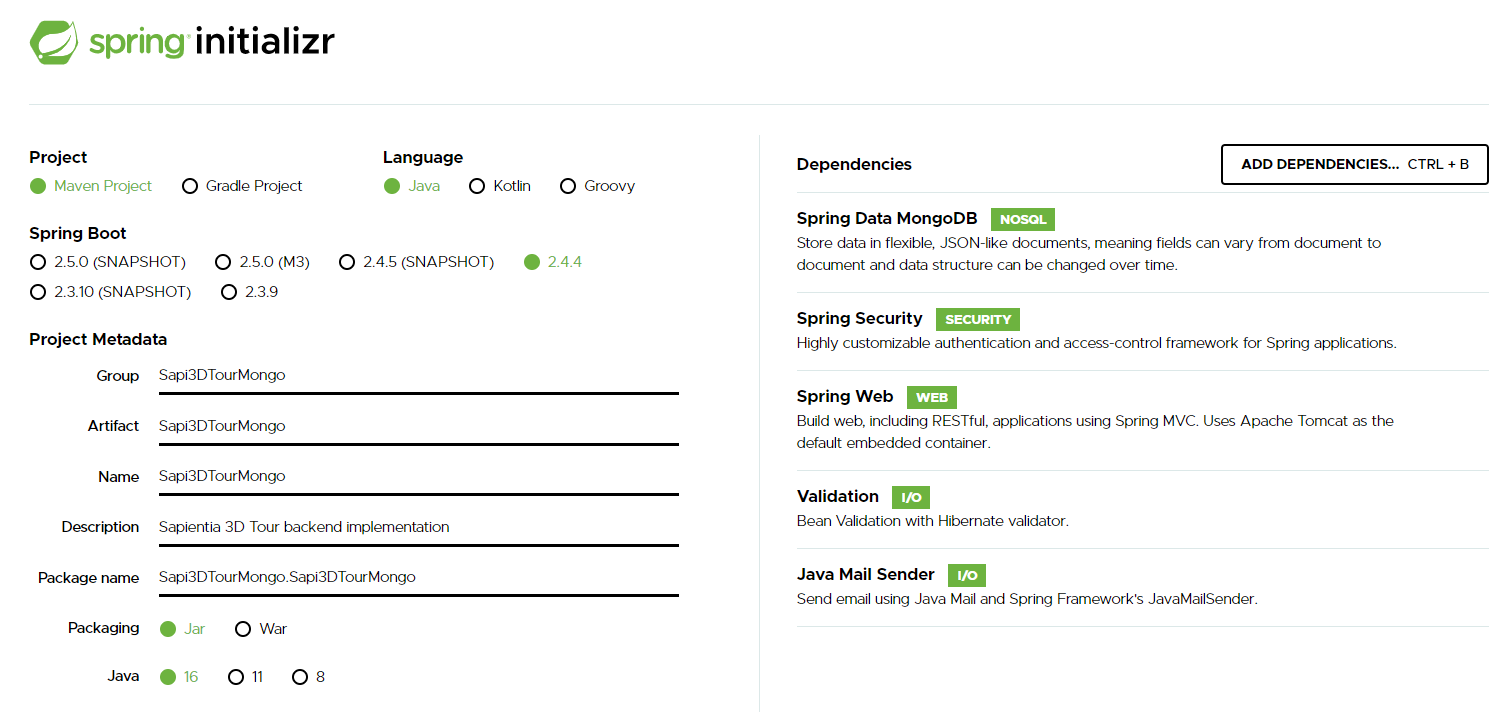
\includegraphics[width=0.8\linewidth]{figures/images/springInit.png}
	\caption[Példa a Spring Initializr használatára]{\textit{Példa a Spring Initializr használatára}}
	\label{fig:springInit}
\end{figure}

\subsection{Adatbázis}
Az adatbázis MongoDB NoSql lett, amelyet az operációs rendszernek megfelelő Workbench-ben kezeltem. Mivel az adatokat nem lehet egy séma alapján felállítani ezért van szükség a NoSQL adatbázisra.

Az adatbázis létrehozásához a következő lépéseket végeztem el:
\begin{itemize}
	\item Telepítettem a MongoDB adatbázis kezelő rendszert.
	\item A MongoDB-hez tartozó Workbench telepítése
	\item Létrehoztam az adatbázist a Workbench segítségével
	\item Kollekciókat nem itt hoztam létre. Az a Spring Boot feladata.
\end{itemize}